\documentclass[a4,12pt]{scrartcl}

%Basic 
\usepackage[utf8]{inputenc}
\usepackage[ngerman]{babel}
\usepackage[T1]{fontenc}
%Schrift 
%\usepackage{fontspec} 
%\setmainfont{Arial} 
%Zeilenabstand
\usepackage{setspace}
\setstretch {1.3}
\usepackage{float}
\usepackage[bottom = 3.50cm]{geometry}

%Titel Seite
\usepackage{titling} %Wird benötigt damit \maketitle die Variabeln title, author und date nicht überschreibt
\title{Test Cases}
%\subtitle{Projekt: software name}
\author{David Meister \and Andreas Stalder}		
 %mit /and können Personen hinzugefügt werden
\date{\today}


%Kopf, Fusszeile
\usepackage{fancyhdr}
\pagestyle{fancy}
\lhead{}
\chead{}
\rhead{Requirements}
\lfoot{\thetitle \: v1.0 }
\cfoot{\today}
\rfoot{Seite \thepage}
\renewcommand{\headrulewidth}{0.4pt}

%Bilder
\usepackage{graphicx}

%Zeichnen
\usepackage{tikz}

%Tabellen
\usepackage{booktabs}
\usepackage{longtable}

%Codesnippets
\usepackage{listings}
\lstset{language=java,basicstyle=\footnotesize,frame=single} %backgroundcolor=\color{lightgray}

%Querformat für eine Seite
\usepackage{lscape}
\usepackage{rotating}
\usepackage{pdflscape}

%URL 
\usepackage[colorlinks=true, linkcolor=blue, urlcolor=blue, citecolor=blue]{hyperref}
\urlstyle{same} 


%Loremimpsum
\usepackage{lipsum}



\begin{document}

%\clearpage\maketitle
\begin{titlepage}
	\centering
	\vspace{5cm}
	\begin{center}
%	\includegraphics[width=0.50\textwidth]{}
	\end{center}
%	{\huge\bfseries software name\par}
	\vspace{8cm}
	\raggedright
	{\bfseries HSR Studienarbeit Network Unit Testing\par}
	{\huge\bfseries Requirements\par}
	\vspace{1cm}
	{\theauthor \par}
	{\today\par}

\end{titlepage}

\section{Änderungsgeschichte}

\begin{table}[htb]
\centering
    \begin{tabular}{@{} l l l l@{}}\toprule    
    {Datum} & {Version} & {Änderung} & {Autor}\\ \midrule
    10.10.16 & 1.0 & Erstellung erster Version & dm/as\\ \addlinespace
    \end{tabular}
\caption{\textbf{Änderungsgeschichte}}
\end{table}

\newpage

%\thispagestyle{empty}
\tableofcontents
\newpage


\section{Einführung}
\subsection{Zweck}
Dieses Dokument beschreibt die Anforderungen mittels Use Cases und nichtfunktionalen
Anforderungen.
\subsection{Gültigkeitsbereich}
Dieses Dokument ist über die gesamte Projektdauer gültig. Es wird in späteren Iterationen angepasst. Somit ist jeweils die neuste Version des Dokuments gültig und alte Versionen sind obsolet.
\subsection{Referenzen}
- Network Testing Analyse
- Network Testing Detailed

\newpage
\section{Allgemeine Beschreibung}
\subsection{Produktperspektive}
Mit Network Unit Tests wird ein automatisches und wiederholbares Testing Framework für Netzwerkumgebungen bereitgestellt. Das Testing der Funktionalitäten im Netzwerk wird meist manuell ausgeführt. Oft werden wichtige Tests vergessen und dadurch Fehler produziert. Mittels automatischem Testen soll ein Werkzeug bereitgestellt werden, um diese Problematik einzudämmen.
\subsection{Produkfunktionen}
Das Programm soll den Anwendern erlauben, Testszenarien zu konfigurieren, auszuführen und auszuwerten. Diese Testszenarien sollen wiederholbar sein, damit sie nach wichtigen Änderungen im Netz einfach ausgeführt werden können.
\subsection{Benutzer Charakteristik}
Zielpersonen sind Netzwerk Engineers, System Administratoren und weitere Informatiker mit Tätigkeit im Netzwerkbereich. Es werden solide Grundkenntnisse in IP-Netzwerken sowie Kenntnisse der verwendeten Netzwerk Devices vorausgesetzt. Der Anwender muss das zu testende Netzwerk im Detail kennen. 
\subsection{Einschränkungen}
Die Software wird auf Linux Plattformen unterstützt. Vorerst werden nur Cisco Netzwerkdevices und Linux Server als zu testende Devices unterstützt.
\newpage
\section{Use Cases}
\subsection{Use Cases Diagramm}
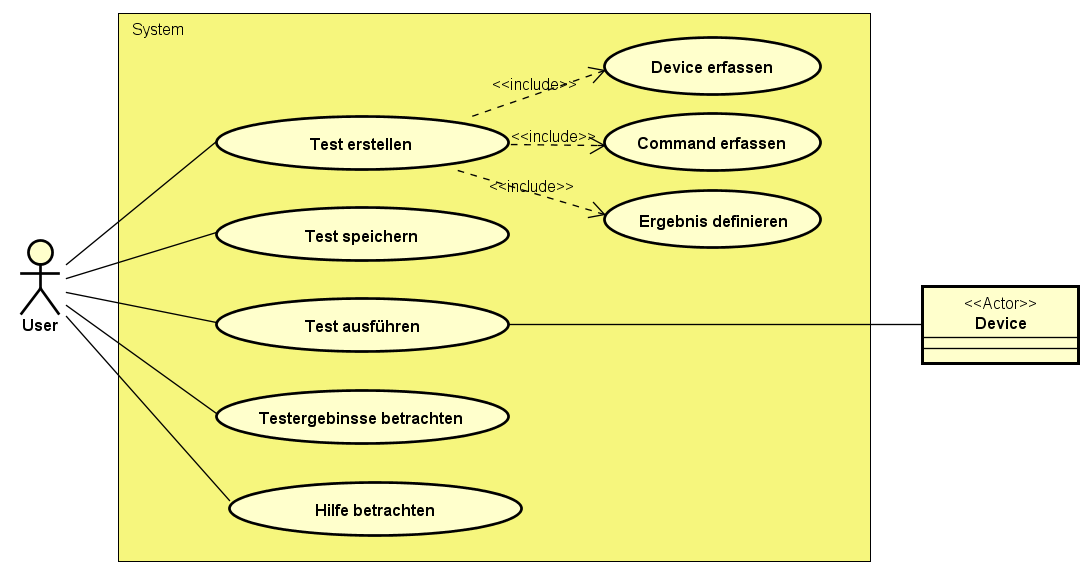
\includegraphics[scale=0.52]{figures/UseCase_Diagram}
\subsection{Aktoren}
\subsection{Beschreibungen}

\newpage
\section{Nichtfunktionale Anforderungen}

\end{document}

